\documentclass[12pt]{article}
\usepackage[top=2cm, bottom=2cm, left=2cm, right=2cm]{geometry}
\usepackage{graphicx,url,tikz}
\usepackage{amssymb,amsmath,amsthm,amsfonts}
\newtheorem{theorem}{Theorem}
\usetikzlibrary{arrows,decorations.markings}
\tikzstyle{vertex}=[circle, draw, inner sep=1pt, minimum size=8pt]
\newcommand{\pic}[1]{{\footnotesize\tt #1}}
\newcommand{\vertex}{\node[vertex]}
\newcommand{\ttld}{{\textasciitilde}}
\pagestyle{plain}
\setlength{\parskip}{.5em}
%\includeonly{s.prune}
\begin{document}
\hfill{\Large\bf cmput 396 ~ solving linear go ~ prof hayward}\hfill~

\section*{linear go}
We discuss briefly
the problem of solving go on small boards.
We consider
{\bf linear go}, ie.\ go on a 1$\times$$n$ board, for some $n$.
We will consider the simplest go rule set:
Tromp-Taylor (so, positional superko)
with no suicide (so, each move is either pass,
or a play that leaves the stone played in a group
that has at least one liberty).

Anyone can solve any go position, given enough time and space:
just build the complete minimax search tree.
But, as you can see from the examples below, the
game trees can get large, so our goal is
to use efficient algorithms and
{\bf to prune child moves that do not change the 
parent's minimax value}.

Here is the game tree for 1x2 go with, 
at each node, isomorphic children pruned.

\[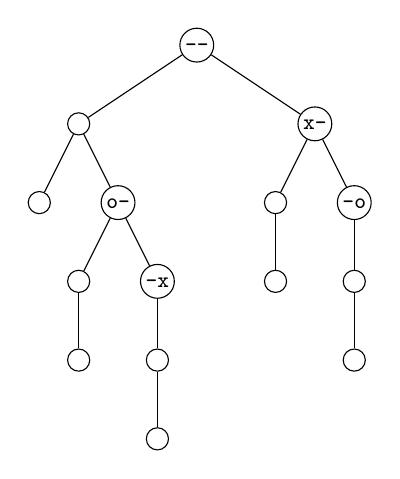
\begin{tikzpicture}[x=1cm, y=1cm
  ,every edge/.style={draw, postaction={decorate,decoration={markings,}}}
]
\vertex (a) at (5,9) {\pic{--}};
\vertex (b) at (3.5,8) { };
\vertex (c) at (6.5,8) {\pic{x-}};
\vertex (d) at (3,7) { };
\vertex (e) at (4,7) {\pic{o-}};
\vertex (f) at (6,7) { };
\vertex (g) at (7,7) {\pic{-o}};
\vertex (h) at (3.5,6) { };
\vertex (i) at (4.5,6) {\pic{-x}};
\vertex (j) at (6,6) {};
\vertex (k) at (7,6) {};
\vertex (l) at (3.5,5) {};
\vertex (m) at (4.5,5) {};
\vertex (n) at (7,5) {};
\vertex (o) at (4.5,4) {};
\path
(a) edge (b) edge (c)
(b) edge (d) edge (e)
(c) edge (f) edge (g)
(e) edge (h) edge (i)
(f) edge (j)
(g) edge (k)
(h) edge (l)
(i) edge (m)
(k) edge (n)
(m) edge (o)
;
\end{tikzpicture}\]

Here is the game tree (top 3 levels only)
for 1x3 go with, at each node, isomorphic children pruned.
On the diagram, draw the next level of the tree.
Then, on the diagram,
label each node with the first-player minimax score.

\[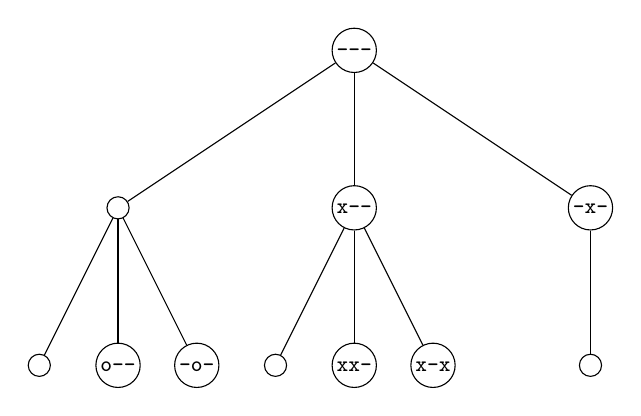
\begin{tikzpicture}[x=1cm, y=2cm
  ,every edge/.style={draw, postaction={decorate,decoration={markings,}}}
]
\vertex (a) at (5,9) {\pic{---}};
\vertex (b) at (2,8) { };
\vertex (c) at (5,8) {\pic{x--}};
\vertex (d) at (8,8) {\pic{-x-}};
\vertex (e) at (1,7) { };
\vertex (f) at (2,7) {\pic{o--}};
\vertex (g) at (3,7) {\pic{-o-}};
\vertex (h) at (4,7) { };
\vertex (i) at (5,7) {\pic{xx-}};
\vertex (j) at (6,7) {\pic{x-x}};
\vertex (k) at (8,7) { };
\path
(a) edge (b) edge (c) edge (d)
(b) edge (e) edge (f) edge (g)
(c) edge (h) edge (i) edge (j)
(d) edge (k)
;
\end{tikzpicture}\]
\vfill~

\section*{early win detection}
One way to prune moves is with {\bf early win detection:}
recognize the final minimax score before
the final state is reached.
For example, 
sometimes it can be seen by examining a position
that, regardless of the game history
(which can make moves illegal by the superko rule),
white has no legal moves.


One form of win detection uses {\bf Benson-safe positions}.
We will call a linear go position {\bf black Benson-safe}
if from that position, regardless
of game history,
the only legal white move is pass.
\noindent
{\bf observe: ~}

{\bf for any shape empty go board,
the first-player minimax score $t$ is non-negative.}

\noindent
{\bf proof. ~}
use strategy stealing.
argue by contradiction:
assume $t$ negative.
consider game after first move is pass.
now opponent has empty board.
~
case 1: opponent passes, game ends, score 0.
~
case 2: opponent does not pass.
from this point, after exchanging 
the names of the players,
the game tree is identical to the
original game tree,
so opponent's minimax score is $t < 0$,
so opponent prefers case 1, pass, minimax score 0.
~
so, from original position,
first player has a move (pass) with minimax score 0,
which is greater than the minimax score $t$, contradiction.
~ qed.
\vfill

\noindent
{\bf similarly:}

{\bf for any shape empty go board,
let first-player minimax score be $t$.
then first-player minimax score
after first move pass is $-t$.}
~ 
we leave the proof as an exercise.
\vfill

\[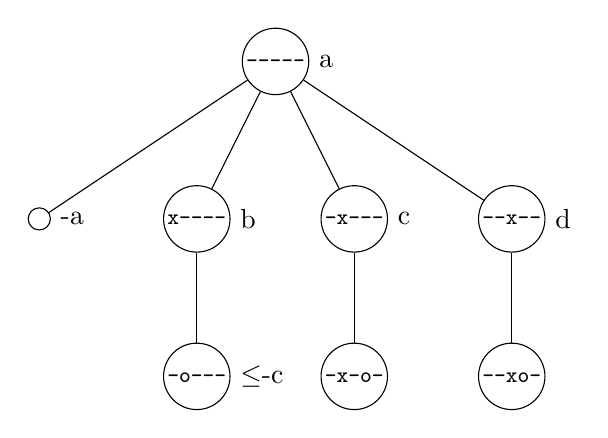
\begin{tikzpicture}[x=1cm, y=2cm
  ,every edge/.style={draw, postaction={decorate,decoration={markings,}}}
]
\vertex (a) at (5,10) [label=right:a]{\pic{-----}};
\vertex (b) at (2, 9) [label=right:-a]{ };
\vertex (c) at (4, 9) [label=right:b]{\pic{x----}};
\vertex (d) at (6, 9) [label=right:c]{\pic{-x---}};
\vertex (e) at (8, 9) [label=right:d]{\pic{--x--}};
\vertex (f) at (4, 8) [label=right:$\leq$-c]{\pic{-o---}};
\vertex (g) at (6, 8) {\pic{-x-o-}};
\vertex (h) at (8, 8) {\pic{--xo-}};
\path
(a) edge (b) edge (c) edge (d) edge (e)
(c) edge (f)
(d) edge (g)
(e) edge (h)
;
\end{tikzpicture}\]
\vfill~

\section*{a pruning theorem}
Here, we discuss go assuming no-suicide Tromp-Taylor rules,
so with the positional superko rule.

So, define the {\em history} of a go state as the sequence
$\mP = (P_0, \ldots, P_{t-1})$
of board positions $P_j$, 
where $P_0$ and $P_{t-1}$ 
are respectively the original and current position,
and $|\mP| = t$ is the number of positions in the history.
Define a {\em go state} $S=(\mP,x)$ by its history $\mP$
and by the player to move (ptm) $x$.

Label the cells of the linear go board from 0 to $n-1$
in the obvious way, ie.\ so that,
for $1 \leq j \leq n-1$, cells $j-1$ and $j$ are neighbours.

For a go state $S$, 
$\mu_x(S)$ is the minimax value for $x$ of $S$.

For cells $x,y$ of a position $P$,
the {\em x,y-interchange} $\phi(x,y,P)$ of $P$ is
the position $P'$ obtained from $P$ by 
interchanging the contents of cells $x$ and $y$.
For example,
let $P$ be the linear go position {\tt ( x - o o - ) }.
Then $\phi(0,1,P)$ is the position {\tt ( - x o o - ) }.

Similarly,
the {\em x,y-interchange} $\phi(x,y,\mP)$ of $\mP$
is the history $\mP'$ obtained from $S$ by interchanging
the contents of cells $x$ and $y$ in each position $P_j$ of $\mP$.

\begin{theorem}
Let $S^0 =(\mP,z)$ be a go state in which the current position
$P_j$ has cell 0 $x$ and cell 1 empty.
Let $\mP' = \phi(0,1,\mP)$, and let
$S^1 = (\mP',z)$ be a valid go state, ie.\ the sequence
of positions in $S_1$ corresponds to a sequence of legal moves.
Then $\mu_x(S^0) \leq \mu_x(S^1)$.
\end{theorem}

We will sometimes represent positions pictorially:
eg.\ ({\tt x - }$\rho$) is a position with cell 0 x, cell 1 empty,
and remaining cell sequence $\rho$.

~

\begin{proof}
The current positions of $S^0$ and $S^1$ are respectively
({\tt x - }$\rho$) and ({\tt - x }$\rho$).
We want to find the minimax value for x of $S^0$ and $S^1$,
so let the player-to-move z be o, the opponent of x. 

First assume that $S_0$ is a terminal state:
the last move was pass, as was the immediately previous move by x.
Notice that this implies $S_1$ is also terminal.
Here, the minimax value is just the Tromp-Taylor score:
if the first non-empty cell in $\rho$ is x, $\mu_x(S_0)=\mu_x(S_1)$;
if not, $\mu_x(S_0) = \mu_x(S_1) - 1$.
So the theorem holds.

Next assume that neither $S_0$ nor $S_1$ are terminal.
Let $L^0$ and $L^1$
be the set of legal moves for o from $S^0$ and $S^1$ respectively.
$\mP'$ is the 0,1-interchange of $\mP$,
so $L^0 - \{0,1\} = L^* = L^1 - \{0,1\}$.

From $S^0$,
the move by o to cell 1 captures the x in cell 0,
so 1 is in $L^0$ if and only if the resulting position
({\tt - - }$\rho'$) is not in $\mP$,
where $\rho' = \rho$ unless $\rho$ begins with a sequence
$\sigma$ of consecutive x's followed by either o or the end of the board,
in which case these x's are also captured when o plays at cell 1.

Now consider from $S^1$ the move by o to cell 0.
If $\rho' = \rho$, then $\rho$ does not begin with a sequence $\sigma$
as described above, and this move does not capture the x
at cell 1, so this move is not legal.
Also, if $\rho' \neq \rho$, then
$\rho$ does begin with $\sigma$,
and so the position after o captures the x's at cells \{1\} 
and the locations of $\sigma$ will be exactly the same,
except for interchanging cells 0 and 1,
as the position after o captures the x's by playing at cell 1 from $S^0$.
So, since $\mP'$ is the 0,1-interchange of $\mP$,
if this move by o from $S^1$ to cell 0 is legal,
the so is the move by 1 from $S^0$ to cell 1.

So there are 3 cases:
$L^0 = L^* = L_1$;
$L^0 = L^* \cup \{1\}, L_1 = L*$;
$L^0 = L^* \cup \{1\}, L_1 = L* \cup \{0\}$.

In each case, observe that for every cell $c$ in $L^*$,
the position $Q_0$ obtained from the o-move to c from $S^0$ 
is the 0,1-interchange of 
the position $Q_1$ obtained from the o-move to c from $S^1$.
Also, the hypotheses of the theorem apply to $Q_0$ and $Q_1$,
so by induction we can assume that
$\mu_x(Q_0) \leq \mu_x(Q_1)$.
In the first case, $\mu_x(S_j) = \min_c \{\mu_x(Q_j)\}$
for each $j=0,1$, so
\[ \mu_x(S_0) \: = \: 
\min_c \{\mu_x(Q_0)\} \: \leq \:
\min_c \{\mu_x(Q_1)\} \: = \: 
\mu(S_1) \: , \]
and we are done.
In the second case, $L^0$ contains all the moves of $L^1$,
and one more, which has minimax value say $r$, so
\[ \mu_x(S_0) \: = \: 
\min \{ \: \min_c \{\mu_x(Q_0)\} \; , r \: \} \:  \leq \: 
\min_c \{\mu_x(Q_1)\} \: = \: 
\mu(S_1) \: , \]
and again we are done.
In the third case,
let $V_1$ ($V_0$) be the position
obtained by an o-move from $S_0$ ($S_1$) to cell 1 (cell 0),
let $\mu_o(V_1)$, let $r_0 = \mu_o(V_0)$.
The hypotheses of the theorem apply after exchanging o for x,
so $\mu_o(V_0) \leq \mu_o(V_1)$ by induction.
Also, for any position $A$, $\mu_o(R) = - \mu_x(R)$,
so $r_1 = \mu_x(V_1) \leq \mu_x(V_0) = r_0$, and we have
\[ \mu_x(S_0) \: = \: 
\min \{ \: \min_c \{\mu_x(Q_0)\} \; , r_1 \: \} \: \leq \: 
\min \{ \: \min_c \{\mu_x(Q_1)\} \; , r_0 \: \} \: = \:
\mu(S_1) \: . \]
\end{proof}


\begin{corollary}\label{cor}
For some $k\geq 1$,
let $S=(\mP,x)$ be a linear go state
such that the set of empty cells to which
$x$ has a legal move includes both $0$ and $1$.
Then the minimax value for $x$ for the move to $1$
is at least as good as the minimax value for the move to 0.
\end{corollary}

\begin{theorem}
For $k\geq 1$,
let $S^0 =(\mP,z)$ be a go state in which the current position
$P_j$ has cells $\{0,\ldots,k-1\}$ $x$ and cell $k$ empty.
Let $\mP' = \phi(0,k,\mP)$, and let
$S^1 = (\mP',z)$ be a valid go state, ie.\ the sequence
of positions in $S_1$ corresponds to a sequence of legal moves.
Then $\mu_x(S^0) \leq \mu_x(S^1)$.
\end{theorem}

\begin{proof}
The two positions here correspond to the positions obtained by
inserting $k-1$ x's between cells 0 and 1 
of the two positions of the previous theorem.
The proof is the same.
\end{proof}

\begin{corollary}\label{cor2}
For some $k\geq 1$,
let $S=(\mP,x)$ be a linear go state
such that the current position has x at cells 1,\ldots, k,
and the set of empty cells to which
$x$ has a legal move includes both $0$ and $k+1$.
Then the minimax value for $x$ for the move to $k+1$
is at least as good as the minimax value for the move to 0.
\end{corollary}
\vfill~

We can use the corollaries to prune moves when solving states.
Let us solve the initial position of 1$\times$4 go.
Up to ismorphism symmetry, there are 3 initial moves to consider:
pass, cell 0, cell 1.

\[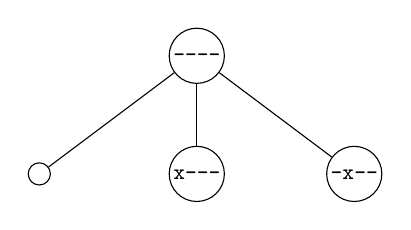
\begin{tikzpicture}[x=1cm, y=1.5cm
  ,every edge/.style={draw, postaction={decorate,decoration={markings,}}}
]
\vertex (a) at (5,9) {\pic{----}};
\vertex (b) at (3,8) { };
\vertex (c) at (5,8) {\pic{x---}};
\vertex (d) at (7,8) {\pic{-x--}};
\path
(a) edge (b) edge (c) edge (d)
;
\end{tikzpicture}\]

By Corollary~\ref{cor}, the move to 
{\tt (- x - -)} is at least as good
as the move to 
{\tt (x - - -)}, so we prune the latter move.
Now let us explore the next levels from {\tt (- x - -)}.

\[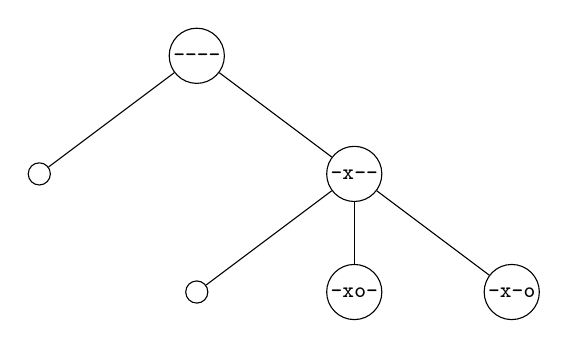
\begin{tikzpicture}[x=1cm, y=1.5cm
  ,every edge/.style={draw, postaction={decorate,decoration={markings,}}}
]
\vertex (a) at (5,9) {\pic{----}};
\vertex (b) at (3,8) { };
\vertex (d) at (7,8) {\pic{-x--}};
\vertex (e) at (5,7) { };
\vertex (f) at (7,7) {\pic{-xo-}};
\vertex (g) at (9,7) {\pic{-x-o}};
\path
(a) edge (b) edge (d)
(d) edge (e) edge (f) edge (g)
;
\end{tikzpicture}\]

Now we can prune {\tt (- x - o)}.
\[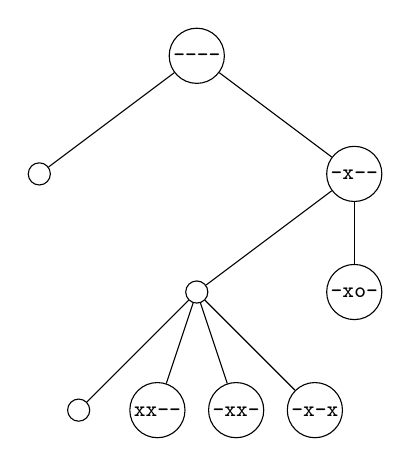
\begin{tikzpicture}[x=1cm, y=1.5cm
  ,every edge/.style={draw, postaction={decorate,decoration={markings,}}}
]
\vertex (a) at (5,9) {\pic{----}};
\vertex (b) at (3,8) { };
\vertex (d) at (7,8) {\pic{-x--}};
\vertex (e) at (5,7) { };
\vertex (f) at (7,7) {\pic{-xo-}};
\vertex (h) at (3.5,6) { };
\vertex (i) at (4.5,6) {\pic{xx--}};
\vertex (j) at (5.5,6) {\pic{-xx-}};
\vertex (k) at (6.5,6) {\pic{-x-x}};
%\vertex (l) at (8,6) {\pic{-x-x}};
\path
(a) edge (b) edge (d)
(d) edge (e) edge (f)
(e) edge (h) edge (i) edge (j) edge (k)
;
\end{tikzpicture}\]
By Corollary~\ref{cor2},
we can prune {\tt (x x - -)}.
By Corollary~\ref{cor},
we can prune {\tt (- x - x)}.
\[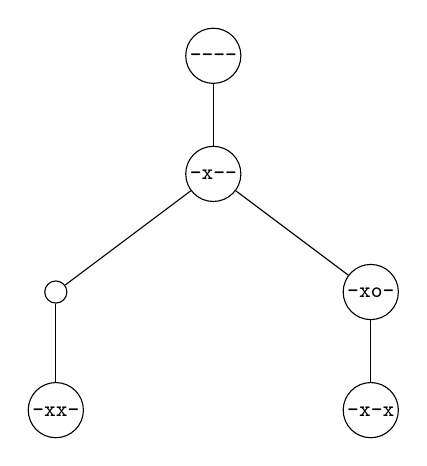
\begin{tikzpicture}[x=1cm, y=1.5cm
  ,every edge/.style={draw, postaction={decorate,decoration={markings,}}}
]
\vertex (a) at (5,9) {\pic{----}};
\vertex (d) at (5,8) {\pic{-x--}};
\vertex (e) at (3,7) { };
\vertex (f) at (7,7) {\pic{-xo-}};
\vertex (j) at (3,6) {\pic{-xx-}};
\vertex (l) at (7,6) {\pic{-x-x}};
\path
(a) edge (d)
(d) edge (e) edge (f)
(e) edge (j)
(f) edge (l)
;
\end{tikzpicture}\]
Here is the final proof tree:
for each x-turn, we show a best move;
for each o-turn, we show all non-pruned moves.
The minimax score for x is 4.

\section*{problem with proof}
proof becomes messy if good move captures

eg

\begin{verbatim}
- - o o o o x - sigma, 2 replies are

- x - - - - x - sigma     <- good move
x - o o o o x - sigma     <- bad move
\end{verbatim}

problem: opponent has more options after good move.

can refill captured area, we have no way to decide
what to do... 2 options:

a) pass in response to each move
into captured set  

b) if there is a unique response to 
an evetual move by o to cell 2, then just play that way

observation:
if we assume cells 1 and 2 have never been played,
then when the stones at 3,4,5,6 in this example were played,
it was for each the 1st time those cells were occupied
(because capture would require that cell 2 be played at)

\end{document}
